\documentclass[twoside]{book}

% Packages required by doxygen
\usepackage{calc}
\usepackage{doxygen}
\usepackage{graphicx}
\usepackage[utf8]{inputenc}
\usepackage{makeidx}
\usepackage{multicol}
\usepackage{multirow}
\usepackage{textcomp}
\usepackage[table]{xcolor}

% Font selection
\usepackage[T1]{fontenc}
\usepackage{mathptmx}
\usepackage[scaled=.90]{helvet}
\usepackage{courier}
\usepackage{amssymb}
\usepackage{sectsty}
\renewcommand{\familydefault}{\sfdefault}
\allsectionsfont{%
  \fontseries{bc}\selectfont%
  \color{darkgray}%
}
\renewcommand{\DoxyLabelFont}{%
  \fontseries{bc}\selectfont%
  \color{darkgray}%
}

% Page & text layout
\usepackage{geometry}
\geometry{%
  a4paper,%
  top=2.5cm,%
  bottom=2.5cm,%
  left=2.5cm,%
  right=2.5cm%
}
\tolerance=750
\hfuzz=15pt
\hbadness=750
\setlength{\emergencystretch}{15pt}
\setlength{\parindent}{0cm}
\setlength{\parskip}{0.2cm}
\makeatletter
\renewcommand{\paragraph}{%
  \@startsection{paragraph}{4}{0ex}{-1.0ex}{1.0ex}{%
    \normalfont\normalsize\bfseries\SS@parafont%
  }%
}
\renewcommand{\subparagraph}{%
  \@startsection{subparagraph}{5}{0ex}{-1.0ex}{1.0ex}{%
    \normalfont\normalsize\bfseries\SS@subparafont%
  }%
}
\makeatother

% Headers & footers
\usepackage{fancyhdr}
\pagestyle{fancyplain}
\fancyhead[LE]{\fancyplain{}{\bfseries\thepage}}
\fancyhead[CE]{\fancyplain{}{}}
\fancyhead[RE]{\fancyplain{}{\bfseries\leftmark}}
\fancyhead[LO]{\fancyplain{}{\bfseries\rightmark}}
\fancyhead[CO]{\fancyplain{}{}}
\fancyhead[RO]{\fancyplain{}{\bfseries\thepage}}
\fancyfoot[LE]{\fancyplain{}{}}
\fancyfoot[CE]{\fancyplain{}{}}
\fancyfoot[RE]{\fancyplain{}{\bfseries\scriptsize Generated on Tue Feb 4 2014 01\-:09\-:24 for My Project by Doxygen }}
\fancyfoot[LO]{\fancyplain{}{\bfseries\scriptsize Generated on Tue Feb 4 2014 01\-:09\-:24 for My Project by Doxygen }}
\fancyfoot[CO]{\fancyplain{}{}}
\fancyfoot[RO]{\fancyplain{}{}}
\renewcommand{\footrulewidth}{0.4pt}
\renewcommand{\chaptermark}[1]{%
  \markboth{#1}{}%
}
\renewcommand{\sectionmark}[1]{%
  \markright{\thesection\ #1}%
}

% Indices & bibliography
\usepackage{natbib}
\usepackage[titles]{tocloft}
\setcounter{tocdepth}{3}
\setcounter{secnumdepth}{5}
\makeindex

% Hyperlinks (required, but should be loaded last)
\usepackage{ifpdf}
\ifpdf
  \usepackage[pdftex,pagebackref=true]{hyperref}
\else
  \usepackage[ps2pdf,pagebackref=true]{hyperref}
\fi
\hypersetup{%
  colorlinks=true,%
  linkcolor=blue,%
  citecolor=blue,%
  unicode%
}

% Custom commands
\newcommand{\clearemptydoublepage}{%
  \newpage{\pagestyle{empty}\cleardoublepage}%
}


%===== C O N T E N T S =====

\begin{document}

% Titlepage & ToC
\hypersetup{pageanchor=false}
\pagenumbering{roman}
\begin{titlepage}
\vspace*{7cm}
\begin{center}%
{\Large My Project }\\
\vspace*{1cm}
{\large Generated by Doxygen 1.8.6}\\
\vspace*{0.5cm}
{\small Tue Feb 4 2014 01:09:24}\\
\end{center}
\end{titlepage}
\clearemptydoublepage
\tableofcontents
\clearemptydoublepage
\pagenumbering{arabic}
\hypersetup{pageanchor=true}

%--- Begin generated contents ---
\chapter{Hierarchical Index}
\section{Class Hierarchy}
This inheritance list is sorted roughly, but not completely, alphabetically\-:\begin{DoxyCompactList}
\item \contentsline{section}{ai\-Player}{\pageref{classai_player}}{}
\item \contentsline{section}{Audio\-Player}{\pageref{class_audio_player}}{}
\item \contentsline{section}{Data\-Base\-Access\-Class}{\pageref{class_data_base_access_class}}{}
\item Q\-Dialog\begin{DoxyCompactList}
\item \contentsline{section}{Dialog}{\pageref{class_dialog}}{}
\end{DoxyCompactList}
\item Q\-Graphics\-Ellipse\-Item\begin{DoxyCompactList}
\item \contentsline{section}{Chip}{\pageref{class_chip}}{}
\end{DoxyCompactList}
\item Q\-Graphics\-Pixmap\-Item\begin{DoxyCompactList}
\item \contentsline{section}{My\-Field}{\pageref{class_my_field}}{}
\end{DoxyCompactList}
\item Q\-Graphics\-Scene\begin{DoxyCompactList}
\item \contentsline{section}{My\-Graphics\-Scene}{\pageref{class_my_graphics_scene}}{}
\end{DoxyCompactList}
\item Q\-Graphics\-View\begin{DoxyCompactList}
\item \contentsline{section}{My\-Graphics\-View}{\pageref{class_my_graphics_view}}{}
\end{DoxyCompactList}
\item Q\-Linear\-Gradient\begin{DoxyCompactList}
\item \contentsline{section}{My\-Gradient}{\pageref{class_my_gradient}}{}
\end{DoxyCompactList}
\item Q\-Object\begin{DoxyCompactList}
\item \contentsline{section}{Chip}{\pageref{class_chip}}{}
\item \contentsline{section}{Connect\-Four}{\pageref{class_connect_four}}{}
\item \contentsline{section}{My\-Field}{\pageref{class_my_field}}{}
\item \contentsline{section}{My\-Gradient}{\pageref{class_my_gradient}}{}
\end{DoxyCompactList}
\item Q\-Property\-Animation\begin{DoxyCompactList}
\item \contentsline{section}{My\-Animation}{\pageref{class_my_animation}}{}
\end{DoxyCompactList}
\end{DoxyCompactList}

\chapter{Class Index}
\section{Class List}
Here are the classes, structs, unions and interfaces with brief descriptions\-:\begin{DoxyCompactList}
\item\contentsline{section}{\hyperlink{classai_player}{ai\-Player} \\*Computergegner für das Spiel. Min\-Max/\-Alpha-\/\-Beta-\/\-Implementierung ist unfertig. möglich sind nur zufällige Züge. }{\pageref{classai_player}}{}
\item\contentsline{section}{\hyperlink{class_audio_player}{Audio\-Player} \\*Simpler Audioplayer. Befindet sich noch in Entwicklung }{\pageref{class_audio_player}}{}
\item\contentsline{section}{\hyperlink{class_chip}{Chip} \\*Spielsteinklasse für das Spielbrett. }{\pageref{class_chip}}{}
\item\contentsline{section}{\hyperlink{class_connect_four}{Connect\-Four} \\*Vier\-Gewinnt-\/\-Logik enthaltende Klasse. Hält den zustand des Spielbrettes und kennt die Regeln des Spiels. Seine Felder werden in der S\-Q\-Lite D\-B persistiert. }{\pageref{class_connect_four}}{}
\item\contentsline{section}{\hyperlink{class_data_base_access_class}{Data\-Base\-Access\-Class} \\*Klasse zum Speichern des Spielzustands in der Datenbank. Benutzt eine S\-Q\-Lite Datenbank. }{\pageref{class_data_base_access_class}}{}
\item\contentsline{section}{\hyperlink{class_dialog}{Dialog} \\*Konfigurationsdialog für Das Spiel. Beim bestätigen werden die Felder zum erzeugen eines Vier Gewinnt Spiels genutzt. Beim Laden werden die Daten aus dem Table\-View genutzt. Das cf\-Game kann dann von außen abgegriffen und verwendet werden. }{\pageref{class_dialog}}{}
\item\contentsline{section}{\hyperlink{class_my_animation}{My\-Animation} \\*Animationsklasse, die sich die Bewegungsrichtung merkt. }{\pageref{class_my_animation}}{}
\item\contentsline{section}{\hyperlink{class_my_field}{My\-Field} \\*Klasse für das Spielbrett. Die Mehrfachvererbung ist für die Animation notwendig }{\pageref{class_my_field}}{}
\item\contentsline{section}{\hyperlink{class_my_graphics_scene}{My\-Graphics\-Scene} \\*Fängt die die Nutzereingaben während des Spiels auf. Kümmert sich um Animationen und Effekte. }{\pageref{class_my_graphics_scene}}{}
\item\contentsline{section}{\hyperlink{class_my_graphics_view}{My\-Graphics\-View} \\*Parentobjekt für die Spielszene. Fängt Tastendrücke ab und achtet auf die Seitenverhältnisse. }{\pageref{class_my_graphics_view}}{}
\end{DoxyCompactList}

\chapter{Class Documentation}
\hypertarget{classai_player}{\section{ai\-Player Class Reference}
\label{classai_player}\index{ai\-Player@{ai\-Player}}
}


Computergegner für das Spiel. Min\-Max/\-Alpha-\/\-Beta-\/\-Implementierung ist unfertig. möglich sind nur zufällige Züge.  




{\ttfamily \#include $<$aiplayer.\-h$>$}

\subsection*{Public Member Functions}
\begin{DoxyCompactItemize}
\item 
\hyperlink{classai_player_a1218587a379bb61445aa5e67a932e262}{ai\-Player} ()
\begin{DoxyCompactList}\small\item\em Setzt den Schwierigkeitslevel. von 0 -\/ 3 \end{DoxyCompactList}\item 
\hypertarget{classai_player_ac815cf510e2c03291e597fa25b732b44}{int {\bfseries Maximize} (Q\-Vector$<$ Q\-Vector$<$ int $>$ $>$ \&board, int turn, int \&alpha, int \&beta)}\label{classai_player_ac815cf510e2c03291e597fa25b732b44}

\item 
\hypertarget{classai_player_a383a7f3c0dd9fedc3bb547658b4da501}{int {\bfseries Minimize} (Q\-Vector$<$ Q\-Vector$<$ int $>$ $>$ \&board, int turn, int \&alpha, int \&beta)}\label{classai_player_a383a7f3c0dd9fedc3bb547658b4da501}

\item 
int \hyperlink{classai_player_a9290bc63d6b1752a44784d8bd75f365b}{get\-Random\-Move} (int colum)
\begin{DoxyCompactList}\small\item\em Liefert einen zufällig generierten Zug zurück. Der Zug bechtet keine ungültigen Züge \end{DoxyCompactList}\item 
\hypertarget{classai_player_a902e0b5e22d6c3ea4bd3e46fdfc2c582}{int {\bfseries Player\-Identifier} ()}\label{classai_player_a902e0b5e22d6c3ea4bd3e46fdfc2c582}

\item 
\hypertarget{classai_player_a030497003f89504920773b788ac91425}{int {\bfseries Other\-Player\-Identifier} ()}\label{classai_player_a030497003f89504920773b788ac91425}

\item 
int \hyperlink{classai_player_a431a9ec4ef7a4072ffac7a3ac3816d8a}{get\-Difficulty} () const 
\begin{DoxyCompactList}\small\item\em Liefert den Schwierigkeitsgrad der K\-I \end{DoxyCompactList}\item 
void \hyperlink{classai_player_a3cdaa5c64f3e7f60559ec2973f578197}{set\-Difficulty} (int value)
\begin{DoxyCompactList}\small\item\em Setzt den Schwierigkeitsgrad der K\-I \end{DoxyCompactList}\item 
\hypertarget{classai_player_a7fca408a282f3e0f9f3f517fe61ebb83}{void {\bfseries set\-Game} (\hyperlink{class_connect_four}{Connect\-Four} $\ast$cfgame)}\label{classai_player_a7fca408a282f3e0f9f3f517fe61ebb83}

\item 
int \hyperlink{classai_player_a5b30b321986ef6a14d6b39b2e6c488e1}{get\-Move} (int column)
\begin{DoxyCompactList}\small\item\em Führt einen Zug entsprechend des gewählten Schwierigskeitsgrades aus. \end{DoxyCompactList}\end{DoxyCompactItemize}


\subsection{Detailed Description}
Computergegner für das Spiel. Min\-Max/\-Alpha-\/\-Beta-\/\-Implementierung ist unfertig. möglich sind nur zufällige Züge. 



\subsection{Constructor \& Destructor Documentation}
\hypertarget{classai_player_a1218587a379bb61445aa5e67a932e262}{\index{ai\-Player@{ai\-Player}!ai\-Player@{ai\-Player}}
\index{ai\-Player@{ai\-Player}!aiPlayer@{ai\-Player}}
\subsubsection[{ai\-Player}]{\setlength{\rightskip}{0pt plus 5cm}ai\-Player\-::ai\-Player (
\begin{DoxyParamCaption}
{}
\end{DoxyParamCaption}
)}}\label{classai_player_a1218587a379bb61445aa5e67a932e262}


Setzt den Schwierigkeitslevel. von 0 -\/ 3 

Liefert eine Instanz auf eine \hyperlink{classai_player}{ai\-Player} Klasse 

\subsection{Member Function Documentation}
\hypertarget{classai_player_a431a9ec4ef7a4072ffac7a3ac3816d8a}{\index{ai\-Player@{ai\-Player}!get\-Difficulty@{get\-Difficulty}}
\index{get\-Difficulty@{get\-Difficulty}!aiPlayer@{ai\-Player}}
\subsubsection[{get\-Difficulty}]{\setlength{\rightskip}{0pt plus 5cm}int ai\-Player\-::get\-Difficulty (
\begin{DoxyParamCaption}
{}
\end{DoxyParamCaption}
) const}}\label{classai_player_a431a9ec4ef7a4072ffac7a3ac3816d8a}


Liefert den Schwierigkeitsgrad der K\-I 

\hypertarget{classai_player_a5b30b321986ef6a14d6b39b2e6c488e1}{\index{ai\-Player@{ai\-Player}!get\-Move@{get\-Move}}
\index{get\-Move@{get\-Move}!aiPlayer@{ai\-Player}}
\subsubsection[{get\-Move}]{\setlength{\rightskip}{0pt plus 5cm}int ai\-Player\-::get\-Move (
\begin{DoxyParamCaption}
\item[{int}]{columns}
\end{DoxyParamCaption}
)}}\label{classai_player_a5b30b321986ef6a14d6b39b2e6c488e1}


Führt einen Zug entsprechend des gewählten Schwierigskeitsgrades aus. 


\begin{DoxyParams}{Parameters}
{\em columns} & Anzahl der Spalten, die zur Verfügung stehen\\
\hline
\end{DoxyParams}
\begin{DoxyReturn}{Returns}
Gewählte Spalte
\end{DoxyReturn}


Here is the call graph for this function\-:


\hypertarget{classai_player_a9290bc63d6b1752a44784d8bd75f365b}{\index{ai\-Player@{ai\-Player}!get\-Random\-Move@{get\-Random\-Move}}
\index{get\-Random\-Move@{get\-Random\-Move}!aiPlayer@{ai\-Player}}
\subsubsection[{get\-Random\-Move}]{\setlength{\rightskip}{0pt plus 5cm}int ai\-Player\-::get\-Random\-Move (
\begin{DoxyParamCaption}
\item[{int}]{columns}
\end{DoxyParamCaption}
)}}\label{classai_player_a9290bc63d6b1752a44784d8bd75f365b}


Liefert einen zufällig generierten Zug zurück. Der Zug bechtet keine ungültigen Züge 


\begin{DoxyParams}{Parameters}
{\em columns} & Anzahl der Spalten, die zur Auswahl stehen\\
\hline
\end{DoxyParams}
\begin{DoxyReturn}{Returns}
Wert der gewählten Spalte
\end{DoxyReturn}


Here is the caller graph for this function\-:


\hypertarget{classai_player_a3cdaa5c64f3e7f60559ec2973f578197}{\index{ai\-Player@{ai\-Player}!set\-Difficulty@{set\-Difficulty}}
\index{set\-Difficulty@{set\-Difficulty}!aiPlayer@{ai\-Player}}
\subsubsection[{set\-Difficulty}]{\setlength{\rightskip}{0pt plus 5cm}void ai\-Player\-::set\-Difficulty (
\begin{DoxyParamCaption}
\item[{int}]{value}
\end{DoxyParamCaption}
)}}\label{classai_player_a3cdaa5c64f3e7f60559ec2973f578197}


Setzt den Schwierigkeitsgrad der K\-I 



Here is the caller graph for this function\-:




The documentation for this class was generated from the following files\-:\begin{DoxyCompactItemize}
\item 
aiplayer.\-h\item 
aiplayer.\-cpp\item 
merge.\-cpp\end{DoxyCompactItemize}

\hypertarget{class_audio_player}{\section{Audio\-Player Class Reference}
\label{class_audio_player}\index{Audio\-Player@{Audio\-Player}}
}


Simpler Audioplayer. Befindet sich noch in Entwicklung  




{\ttfamily \#include $<$audioplayer.\-h$>$}

\subsection*{Public Member Functions}
\begin{DoxyCompactItemize}
\item 
\hypertarget{class_audio_player_afa3f18ddf21af783358873f91cec4783}{void {\bfseries Play} ()}\label{class_audio_player_afa3f18ddf21af783358873f91cec4783}

\end{DoxyCompactItemize}


\subsection{Detailed Description}
Simpler Audioplayer. Befindet sich noch in Entwicklung 



The documentation for this class was generated from the following files\-:\begin{DoxyCompactItemize}
\item 
audioplayer.\-h\item 
audioplayer.\-cpp\item 
merge.\-cpp\end{DoxyCompactItemize}

\hypertarget{class_chip}{\section{Chip Class Reference}
\label{class_chip}\index{Chip@{Chip}}
}


Spielsteinklasse für das Spielbrett.  




{\ttfamily \#include $<$chip.\-h$>$}



Inheritance diagram for Chip\-:


Collaboration diagram for Chip\-:
\subsection*{Public Member Functions}
\begin{DoxyCompactItemize}
\item 
\hyperlink{class_chip_a50f4a36e13f90a93d0a7ed1360bfe92a}{Chip} (int x, int y, int w, int h, int player, Q\-Object $\ast$parent=N\-U\-L\-L)
\begin{DoxyCompactList}\small\item\em Konstruktor der Klasse \hyperlink{class_chip}{Chip}. Erstellt einen Spielstein für Vier Gewinnt \end{DoxyCompactList}\item 
\hyperlink{class_my_animation}{My\-Animation} $\ast$ \hyperlink{class_chip_abb087aff174edd3145895b24f735eb29}{animate} (Q\-Point\-F end, int duration, const Q\-Easing\-Curve \&curve)
\begin{DoxyCompactList}\small\item\em Liefert einen Zeiger auf eine \hyperlink{class_my_animation}{My\-Animation} Instanz zurück, die dann ausgeführt werden kann \end{DoxyCompactList}\item 
int \hyperlink{class_chip_acbf29a18e6349c52878dca3600461af5}{get\-Player} ()
\begin{DoxyCompactList}\small\item\em Liefert den Spieler zurück, der den Stein gelegt hat. \end{DoxyCompactList}\item 
Q\-Point\-F $\ast$ \hyperlink{class_chip_a558787f04d66e87353cf8bebefae1f2d}{get\-Center} ()
\begin{DoxyCompactList}\small\item\em Liefert einen Zeiger auf eine Q\-Point\-F Instanz, die den Mittelpunkt des Objektes beschreibt. \end{DoxyCompactList}\end{DoxyCompactItemize}
\subsection*{Properties}
\begin{DoxyCompactItemize}
\item 
\hypertarget{class_chip_a548329ae211f8de857275407733f2d1f}{Q\-Point\-F {\bfseries pos}}\label{class_chip_a548329ae211f8de857275407733f2d1f}

\end{DoxyCompactItemize}


\subsection{Detailed Description}
Spielsteinklasse für das Spielbrett. 



\subsection{Constructor \& Destructor Documentation}
\hypertarget{class_chip_a50f4a36e13f90a93d0a7ed1360bfe92a}{\index{Chip@{Chip}!Chip@{Chip}}
\index{Chip@{Chip}!Chip@{Chip}}
\subsubsection[{Chip}]{\setlength{\rightskip}{0pt plus 5cm}Chip\-::\-Chip (
\begin{DoxyParamCaption}
\item[{int}]{x, }
\item[{int}]{y, }
\item[{int}]{w, }
\item[{int}]{h, }
\item[{int}]{player, }
\item[{Q\-Object $\ast$}]{parent = {\ttfamily NULL}}
\end{DoxyParamCaption}
)\hspace{0.3cm}{\ttfamily [explicit]}}}\label{class_chip_a50f4a36e13f90a93d0a7ed1360bfe92a}


Konstruktor der Klasse \hyperlink{class_chip}{Chip}. Erstellt einen Spielstein für Vier Gewinnt 


\begin{DoxyParams}{Parameters}
{\em x} & x Position des bounding rect\\
\hline
{\em y} & x Position des bounding rect\\
\hline
{\em w} & Breite Position des bounding rect\\
\hline
{\em h} & Höhe\\
\hline
{\em player} & Spielernummer\\
\hline
{\em parent} & Standardparameter\\
\hline
\end{DoxyParams}


\subsection{Member Function Documentation}
\hypertarget{class_chip_abb087aff174edd3145895b24f735eb29}{\index{Chip@{Chip}!animate@{animate}}
\index{animate@{animate}!Chip@{Chip}}
\subsubsection[{animate}]{\setlength{\rightskip}{0pt plus 5cm}{\bf My\-Animation} $\ast$ Chip\-::animate (
\begin{DoxyParamCaption}
\item[{Q\-Point\-F}]{end, }
\item[{int}]{duration, }
\item[{const Q\-Easing\-Curve \&}]{curve}
\end{DoxyParamCaption}
)}}\label{class_chip_abb087aff174edd3145895b24f735eb29}


Liefert einen Zeiger auf eine \hyperlink{class_my_animation}{My\-Animation} Instanz zurück, die dann ausgeführt werden kann 


\begin{DoxyParams}{Parameters}
{\em end} & Endposition der Animation\\
\hline
{\em duration} & Dauer der Animation\\
\hline
{\em curve} & Zur Beeinflussung des Animationsverhaltens\\
\hline
\end{DoxyParams}
\hypertarget{class_chip_a558787f04d66e87353cf8bebefae1f2d}{\index{Chip@{Chip}!get\-Center@{get\-Center}}
\index{get\-Center@{get\-Center}!Chip@{Chip}}
\subsubsection[{get\-Center}]{\setlength{\rightskip}{0pt plus 5cm}Q\-Point\-F $\ast$ Chip\-::get\-Center (
\begin{DoxyParamCaption}
{}
\end{DoxyParamCaption}
)}}\label{class_chip_a558787f04d66e87353cf8bebefae1f2d}


Liefert einen Zeiger auf eine Q\-Point\-F Instanz, die den Mittelpunkt des Objektes beschreibt. 

\hypertarget{class_chip_acbf29a18e6349c52878dca3600461af5}{\index{Chip@{Chip}!get\-Player@{get\-Player}}
\index{get\-Player@{get\-Player}!Chip@{Chip}}
\subsubsection[{get\-Player}]{\setlength{\rightskip}{0pt plus 5cm}int Chip\-::get\-Player (
\begin{DoxyParamCaption}
{}
\end{DoxyParamCaption}
)}}\label{class_chip_acbf29a18e6349c52878dca3600461af5}


Liefert den Spieler zurück, der den Stein gelegt hat. 



The documentation for this class was generated from the following files\-:\begin{DoxyCompactItemize}
\item 
chip.\-h\item 
chip.\-cpp\item 
merge.\-cpp\end{DoxyCompactItemize}

\hypertarget{class_connect_four}{\section{Connect\-Four Class Reference}
\label{class_connect_four}\index{Connect\-Four@{Connect\-Four}}
}


Vier\-Gewinnt-\/\-Logik enthaltende Klasse. Hält den zustand des Spielbrettes und kennt die Regeln des Spiels. Seine Felder werden in der S\-Q\-Lite D\-B persistiert.  




{\ttfamily \#include $<$connectfour.\-h$>$}



Inheritance diagram for Connect\-Four\-:


Collaboration diagram for Connect\-Four\-:
\subsection*{Public Member Functions}
\begin{DoxyCompactItemize}
\item 
\hyperlink{class_connect_four_a9d7a0db424f22513386fa60ed2d5b575}{Connect\-Four} ()
\begin{DoxyCompactList}\small\item\em Konstruktor der Klasse \hyperlink{class_connect_four}{Connect\-Four}. Die Instanz bildet die Regeln des Spiels Vier Gewinnt ab. \end{DoxyCompactList}\item 
\hyperlink{class_connect_four_ac4fca1dec417914e68e1c8fb22dc87a7}{Connect\-Four} (int x, int y, Q\-String player1\-Name, Q\-String player2\-Name, int difficulty\-Level, int starting\-Player)
\begin{DoxyCompactList}\small\item\em Konstruktor der Klasse \hyperlink{class_connect_four}{Connect\-Four}. Die Instanz bildet die Regeln des Spiels Vier Gewinnt ab. \end{DoxyCompactList}\item 
int \hyperlink{class_connect_four_aab7f413c1f52a8bc9ff21d397f9f1f3f}{set\-Stone} (int x)
\begin{DoxyCompactList}\small\item\em liefert die Zeile zurück, in der der Stein gelandet ist. Prüft, ob der Zug siegreich war. Prüfen mit \hyperlink{class_connect_four_a5b3cc0a97ca9722eb49266e651cdcf3b}{get\-Winner()} \end{DoxyCompactList}\item 
bool \hyperlink{class_connect_four_a38f2e53360ddd8b3152e6583705a1b8a}{check\-Victory} (int x, int y)
\begin{DoxyCompactList}\small\item\em Verschiebt einen Punkt entlang der Linien (diagonal, senkrecht, horizontal) und summiert die Spielerchips auf. \end{DoxyCompactList}\item 
int \hyperlink{class_connect_four_a0916903c07bfbd9891f1203373317e76}{evaluate\-Move} (int x, int y)
\begin{DoxyCompactList}\small\item\em Gibt den größten Wert für \end{DoxyCompactList}\item 
bool \hyperlink{class_connect_four_a70a3cd6ddcc7ae5b1eee3afa64ed6790}{check\-Draw} ()
\begin{DoxyCompactList}\small\item\em Prüft, ob ein unentschieden vorliegt \end{DoxyCompactList}\item 
Q\-String \hyperlink{class_connect_four_afb0b3ab58efa2888c6ee6d5c60df15b7}{get\-Game\-State} ()
\begin{DoxyCompactList}\small\item\em Liefert eine Zeichenkette, die den Spielverlauf darstellt \end{DoxyCompactList}\item 
\hypertarget{class_connect_four_a305120e52fd04399c7e4aa66ede018a2}{void {\bfseries set\-Game\-State} (Q\-String state)}\label{class_connect_four_a305120e52fd04399c7e4aa66ede018a2}

\item 
int \hyperlink{class_connect_four_a9b4b647139235c7c3eae2c5c9c8d7471}{get\-Current\-Player} ()
\begin{DoxyCompactList}\small\item\em Liefert die aktuelle Spielernummer zurück. \end{DoxyCompactList}\item 
bool \hyperlink{class_connect_four_ad00b3add13aac59b6dc6469cb24c7d53}{check\-Move} (int x)
\begin{DoxyCompactList}\small\item\em Prüft, ob ein Zug gültig ist, oder nicht. Wird von der K\-I im einfachen Modus benötigt. 
\begin{DoxyParams}{Parameters}
{\em x} & Gewählte Spalte für den Zug\\
\hline
\end{DoxyParams}
\end{DoxyCompactList}\item 
Q\-String \hyperlink{class_connect_four_a0fb31ff9df21241727dc89111a8237d1}{get\-Name1} () const 
\begin{DoxyCompactList}\small\item\em Liefert den Namen des ersten Spielers \end{DoxyCompactList}\item 
Q\-String \hyperlink{class_connect_four_af1e622aabf4ab9c3e59f120453b4b00a}{get\-Name2} () const 
\begin{DoxyCompactList}\small\item\em Liefert den Namen des zweiten Spielers \end{DoxyCompactList}\item 
\hypertarget{class_connect_four_a1ee5735fdac151d7f11fec3daeeef6fc}{bool {\bfseries get\-Heuristic} () const }\label{class_connect_four_a1ee5735fdac151d7f11fec3daeeef6fc}

\item 
int \hyperlink{class_connect_four_a460f6063899b4e5a7e2171ab310a449b}{get\-Difficulty} () const 
\begin{DoxyCompactList}\small\item\em Feld für den gewählten Schwierigkeitsgrad. \end{DoxyCompactList}\item 
int \hyperlink{class_connect_four_a5b3cc0a97ca9722eb49266e651cdcf3b}{get\-Winner} ()
\begin{DoxyCompactList}\small\item\em Liefert die Spielernummer des Siegers zurück \end{DoxyCompactList}\item 
int \hyperlink{class_connect_four_a88586e2245c07b08979f258bb24c9c17}{get\-Moves} ()
\begin{DoxyCompactList}\small\item\em Liefert die Anzahl der bisherigen Züge zurück \end{DoxyCompactList}\item 
int \hyperlink{class_connect_four_a102316e1b99e7d1eddbe36340ca14544}{get\-Last\-Player} ()
\begin{DoxyCompactList}\small\item\em Liefert die Spielernummer des letzten Zuges zurück. \end{DoxyCompactList}\item 
Q\-String \hyperlink{class_connect_four_aa47ee15206dfa8e942e28ec38428e507}{get\-History} () const 
\begin{DoxyCompactList}\small\item\em Liefert den Spielverlauf in Form einer Zeichenkette zurück. \end{DoxyCompactList}\item 
Q\-String \hyperlink{class_connect_four_af2ba0a09293dccc56439a1f3f76b2c50}{get\-History\-To\-Load} () const 
\begin{DoxyCompactList}\small\item\em Liefert die noch zu ladende Spielehistorie zurück \end{DoxyCompactList}\item 
void \hyperlink{class_connect_four_ab31edf162a4035383b8034f2c65d65b5}{set\-History\-To\-Load} (Q\-String hl)
\begin{DoxyCompactList}\small\item\em Bereitet das Laden eines Spielverlaufs vor. \end{DoxyCompactList}\item 
\hypertarget{class_connect_four_a6a366a01f3c7dcb75441b604df4bed51}{int {\bfseries get\-Starting\-Player} () const }\label{class_connect_four_a6a366a01f3c7dcb75441b604df4bed51}

\end{DoxyCompactItemize}
\subsection*{Public Attributes}
\begin{DoxyCompactItemize}
\item 
\hypertarget{class_connect_four_a69065ab8a638127f0da1d7f284f1e56a}{Q\-Vector$<$ Q\-Vector$<$ int $>$ $>$ {\bfseries board}}\label{class_connect_four_a69065ab8a638127f0da1d7f284f1e56a}

\item 
\hypertarget{class_connect_four_a7507490166cea01cca4562859a01ee8b}{int {\bfseries fieldsx}}\label{class_connect_four_a7507490166cea01cca4562859a01ee8b}

\item 
\hypertarget{class_connect_four_a8da13866381909a976fd12e6b3f2b59c}{int {\bfseries fieldsy}}\label{class_connect_four_a8da13866381909a976fd12e6b3f2b59c}

\item 
\hypertarget{class_connect_four_a7730e7df9fab3346f2bcf43ed4a185f0}{int {\bfseries current\-Player}}\label{class_connect_four_a7730e7df9fab3346f2bcf43ed4a185f0}

\item 
\hypertarget{class_connect_four_a42c3ccb860d071c4307c9d963173b181}{int {\bfseries necessary\-Points\-For\-Winning}}\label{class_connect_four_a42c3ccb860d071c4307c9d963173b181}

\item 
\hypertarget{class_connect_four_a72b70f49c28ba97d33373d3fd398be6a}{Q\-String {\bfseries history}}\label{class_connect_four_a72b70f49c28ba97d33373d3fd398be6a}

\item 
\hypertarget{class_connect_four_a46078d90754278b1048681cc413c9bb3}{Q\-Vector$<$ Q\-Vector$<$ int $>$ $>$ {\bfseries directions}}\label{class_connect_four_a46078d90754278b1048681cc413c9bb3}

\end{DoxyCompactItemize}


\subsection{Detailed Description}
Vier\-Gewinnt-\/\-Logik enthaltende Klasse. Hält den zustand des Spielbrettes und kennt die Regeln des Spiels. Seine Felder werden in der S\-Q\-Lite D\-B persistiert. 



\subsection{Constructor \& Destructor Documentation}
\hypertarget{class_connect_four_a9d7a0db424f22513386fa60ed2d5b575}{\index{Connect\-Four@{Connect\-Four}!Connect\-Four@{Connect\-Four}}
\index{Connect\-Four@{Connect\-Four}!ConnectFour@{Connect\-Four}}
\subsubsection[{Connect\-Four}]{\setlength{\rightskip}{0pt plus 5cm}Connect\-Four\-::\-Connect\-Four (
\begin{DoxyParamCaption}
{}
\end{DoxyParamCaption}
)}}\label{class_connect_four_a9d7a0db424f22513386fa60ed2d5b575}


Konstruktor der Klasse \hyperlink{class_connect_four}{Connect\-Four}. Die Instanz bildet die Regeln des Spiels Vier Gewinnt ab. 

\hypertarget{class_connect_four_ac4fca1dec417914e68e1c8fb22dc87a7}{\index{Connect\-Four@{Connect\-Four}!Connect\-Four@{Connect\-Four}}
\index{Connect\-Four@{Connect\-Four}!ConnectFour@{Connect\-Four}}
\subsubsection[{Connect\-Four}]{\setlength{\rightskip}{0pt plus 5cm}Connect\-Four\-::\-Connect\-Four (
\begin{DoxyParamCaption}
\item[{int}]{x, }
\item[{int}]{y, }
\item[{Q\-String}]{player1\-Name, }
\item[{Q\-String}]{player2\-Name, }
\item[{int}]{difficulty\-Level, }
\item[{int}]{starting\-Player}
\end{DoxyParamCaption}
)}}\label{class_connect_four_ac4fca1dec417914e68e1c8fb22dc87a7}


Konstruktor der Klasse \hyperlink{class_connect_four}{Connect\-Four}. Die Instanz bildet die Regeln des Spiels Vier Gewinnt ab. 


\begin{DoxyParams}{Parameters}
{\em x} & Spalten\\
\hline
{\em y} & Zeileen\\
\hline
{\em player1\-Name} & Name des ersten Spielers\\
\hline
{\em player2\-Name} & Name des zweiten Spielers\\
\hline
{\em difficulty\-Level} & Schwierigkeitsgrad\\
\hline
{\em starting\-Player} & Nummer des beginnenden Spielers\\
\hline
\end{DoxyParams}


\subsection{Member Function Documentation}
\hypertarget{class_connect_four_a70a3cd6ddcc7ae5b1eee3afa64ed6790}{\index{Connect\-Four@{Connect\-Four}!check\-Draw@{check\-Draw}}
\index{check\-Draw@{check\-Draw}!ConnectFour@{Connect\-Four}}
\subsubsection[{check\-Draw}]{\setlength{\rightskip}{0pt plus 5cm}bool Connect\-Four\-::check\-Draw (
\begin{DoxyParamCaption}
{}
\end{DoxyParamCaption}
)}}\label{class_connect_four_a70a3cd6ddcc7ae5b1eee3afa64ed6790}


Prüft, ob ein unentschieden vorliegt 

\hypertarget{class_connect_four_ad00b3add13aac59b6dc6469cb24c7d53}{\index{Connect\-Four@{Connect\-Four}!check\-Move@{check\-Move}}
\index{check\-Move@{check\-Move}!ConnectFour@{Connect\-Four}}
\subsubsection[{check\-Move}]{\setlength{\rightskip}{0pt plus 5cm}bool Connect\-Four\-::check\-Move (
\begin{DoxyParamCaption}
\item[{int}]{x}
\end{DoxyParamCaption}
)}}\label{class_connect_four_ad00b3add13aac59b6dc6469cb24c7d53}


Prüft, ob ein Zug gültig ist, oder nicht. Wird von der K\-I im einfachen Modus benötigt. 
\begin{DoxyParams}{Parameters}
{\em x} & Gewählte Spalte für den Zug\\
\hline
\end{DoxyParams}


\hypertarget{class_connect_four_a38f2e53360ddd8b3152e6583705a1b8a}{\index{Connect\-Four@{Connect\-Four}!check\-Victory@{check\-Victory}}
\index{check\-Victory@{check\-Victory}!ConnectFour@{Connect\-Four}}
\subsubsection[{check\-Victory}]{\setlength{\rightskip}{0pt plus 5cm}bool Connect\-Four\-::check\-Victory (
\begin{DoxyParamCaption}
\item[{int}]{x, }
\item[{int}]{y}
\end{DoxyParamCaption}
)}}\label{class_connect_four_a38f2e53360ddd8b3152e6583705a1b8a}


Verschiebt einen Punkt entlang der Linien (diagonal, senkrecht, horizontal) und summiert die Spielerchips auf. 


\begin{DoxyParams}{Parameters}
{\em x} & x-\/\-Wert des Punktes\\
\hline
{\em y} & y-\/\-Wert des Punktes\\
\hline
\end{DoxyParams}


Here is the caller graph for this function\-:


\hypertarget{class_connect_four_a0916903c07bfbd9891f1203373317e76}{\index{Connect\-Four@{Connect\-Four}!evaluate\-Move@{evaluate\-Move}}
\index{evaluate\-Move@{evaluate\-Move}!ConnectFour@{Connect\-Four}}
\subsubsection[{evaluate\-Move}]{\setlength{\rightskip}{0pt plus 5cm}int Connect\-Four\-::evaluate\-Move (
\begin{DoxyParamCaption}
\item[{int}]{x, }
\item[{int}]{y}
\end{DoxyParamCaption}
)}}\label{class_connect_four_a0916903c07bfbd9891f1203373317e76}


Gibt den größten Wert für 


\begin{DoxyParams}{Parameters}
{\em x} & x-\/\-Wert des Punktes\\
\hline
{\em y} & y-\/\-Wert des Punktes\\
\hline
\end{DoxyParams}
\hypertarget{class_connect_four_a9b4b647139235c7c3eae2c5c9c8d7471}{\index{Connect\-Four@{Connect\-Four}!get\-Current\-Player@{get\-Current\-Player}}
\index{get\-Current\-Player@{get\-Current\-Player}!ConnectFour@{Connect\-Four}}
\subsubsection[{get\-Current\-Player}]{\setlength{\rightskip}{0pt plus 5cm}int Connect\-Four\-::get\-Current\-Player (
\begin{DoxyParamCaption}
{}
\end{DoxyParamCaption}
)}}\label{class_connect_four_a9b4b647139235c7c3eae2c5c9c8d7471}


Liefert die aktuelle Spielernummer zurück. 



Here is the caller graph for this function\-:


\hypertarget{class_connect_four_a460f6063899b4e5a7e2171ab310a449b}{\index{Connect\-Four@{Connect\-Four}!get\-Difficulty@{get\-Difficulty}}
\index{get\-Difficulty@{get\-Difficulty}!ConnectFour@{Connect\-Four}}
\subsubsection[{get\-Difficulty}]{\setlength{\rightskip}{0pt plus 5cm}int Connect\-Four\-::get\-Difficulty (
\begin{DoxyParamCaption}
{}
\end{DoxyParamCaption}
) const}}\label{class_connect_four_a460f6063899b4e5a7e2171ab310a449b}


Feld für den gewählten Schwierigkeitsgrad. 



Here is the caller graph for this function\-:


\hypertarget{class_connect_four_afb0b3ab58efa2888c6ee6d5c60df15b7}{\index{Connect\-Four@{Connect\-Four}!get\-Game\-State@{get\-Game\-State}}
\index{get\-Game\-State@{get\-Game\-State}!ConnectFour@{Connect\-Four}}
\subsubsection[{get\-Game\-State}]{\setlength{\rightskip}{0pt plus 5cm}Q\-String Connect\-Four\-::get\-Game\-State (
\begin{DoxyParamCaption}
{}
\end{DoxyParamCaption}
)}}\label{class_connect_four_afb0b3ab58efa2888c6ee6d5c60df15b7}


Liefert eine Zeichenkette, die den Spielverlauf darstellt 

$<$retuns$>$Zeichenkette mit dem Spielverlauf$<$/retuns$>$ \hypertarget{class_connect_four_aa47ee15206dfa8e942e28ec38428e507}{\index{Connect\-Four@{Connect\-Four}!get\-History@{get\-History}}
\index{get\-History@{get\-History}!ConnectFour@{Connect\-Four}}
\subsubsection[{get\-History}]{\setlength{\rightskip}{0pt plus 5cm}Q\-String Connect\-Four\-::get\-History (
\begin{DoxyParamCaption}
{}
\end{DoxyParamCaption}
) const}}\label{class_connect_four_aa47ee15206dfa8e942e28ec38428e507}


Liefert den Spielverlauf in Form einer Zeichenkette zurück. 



Here is the caller graph for this function\-:


\hypertarget{class_connect_four_af2ba0a09293dccc56439a1f3f76b2c50}{\index{Connect\-Four@{Connect\-Four}!get\-History\-To\-Load@{get\-History\-To\-Load}}
\index{get\-History\-To\-Load@{get\-History\-To\-Load}!ConnectFour@{Connect\-Four}}
\subsubsection[{get\-History\-To\-Load}]{\setlength{\rightskip}{0pt plus 5cm}Q\-String Connect\-Four\-::get\-History\-To\-Load (
\begin{DoxyParamCaption}
{}
\end{DoxyParamCaption}
) const}}\label{class_connect_four_af2ba0a09293dccc56439a1f3f76b2c50}


Liefert die noch zu ladende Spielehistorie zurück 

\hypertarget{class_connect_four_a102316e1b99e7d1eddbe36340ca14544}{\index{Connect\-Four@{Connect\-Four}!get\-Last\-Player@{get\-Last\-Player}}
\index{get\-Last\-Player@{get\-Last\-Player}!ConnectFour@{Connect\-Four}}
\subsubsection[{get\-Last\-Player}]{\setlength{\rightskip}{0pt plus 5cm}int Connect\-Four\-::get\-Last\-Player (
\begin{DoxyParamCaption}
{}
\end{DoxyParamCaption}
)}}\label{class_connect_four_a102316e1b99e7d1eddbe36340ca14544}


Liefert die Spielernummer des letzten Zuges zurück. 

\hypertarget{class_connect_four_a88586e2245c07b08979f258bb24c9c17}{\index{Connect\-Four@{Connect\-Four}!get\-Moves@{get\-Moves}}
\index{get\-Moves@{get\-Moves}!ConnectFour@{Connect\-Four}}
\subsubsection[{get\-Moves}]{\setlength{\rightskip}{0pt plus 5cm}int Connect\-Four\-::get\-Moves (
\begin{DoxyParamCaption}
{}
\end{DoxyParamCaption}
)}}\label{class_connect_four_a88586e2245c07b08979f258bb24c9c17}


Liefert die Anzahl der bisherigen Züge zurück 



Here is the caller graph for this function\-:


\hypertarget{class_connect_four_a0fb31ff9df21241727dc89111a8237d1}{\index{Connect\-Four@{Connect\-Four}!get\-Name1@{get\-Name1}}
\index{get\-Name1@{get\-Name1}!ConnectFour@{Connect\-Four}}
\subsubsection[{get\-Name1}]{\setlength{\rightskip}{0pt plus 5cm}Q\-String Connect\-Four\-::get\-Name1 (
\begin{DoxyParamCaption}
{}
\end{DoxyParamCaption}
) const}}\label{class_connect_four_a0fb31ff9df21241727dc89111a8237d1}


Liefert den Namen des ersten Spielers 



Here is the caller graph for this function\-:


\hypertarget{class_connect_four_af1e622aabf4ab9c3e59f120453b4b00a}{\index{Connect\-Four@{Connect\-Four}!get\-Name2@{get\-Name2}}
\index{get\-Name2@{get\-Name2}!ConnectFour@{Connect\-Four}}
\subsubsection[{get\-Name2}]{\setlength{\rightskip}{0pt plus 5cm}Q\-String Connect\-Four\-::get\-Name2 (
\begin{DoxyParamCaption}
{}
\end{DoxyParamCaption}
) const}}\label{class_connect_four_af1e622aabf4ab9c3e59f120453b4b00a}


Liefert den Namen des zweiten Spielers 



Here is the caller graph for this function\-:


\hypertarget{class_connect_four_a5b3cc0a97ca9722eb49266e651cdcf3b}{\index{Connect\-Four@{Connect\-Four}!get\-Winner@{get\-Winner}}
\index{get\-Winner@{get\-Winner}!ConnectFour@{Connect\-Four}}
\subsubsection[{get\-Winner}]{\setlength{\rightskip}{0pt plus 5cm}int Connect\-Four\-::get\-Winner (
\begin{DoxyParamCaption}
{}
\end{DoxyParamCaption}
)}}\label{class_connect_four_a5b3cc0a97ca9722eb49266e651cdcf3b}


Liefert die Spielernummer des Siegers zurück 



Here is the caller graph for this function\-:


\hypertarget{class_connect_four_ab31edf162a4035383b8034f2c65d65b5}{\index{Connect\-Four@{Connect\-Four}!set\-History\-To\-Load@{set\-History\-To\-Load}}
\index{set\-History\-To\-Load@{set\-History\-To\-Load}!ConnectFour@{Connect\-Four}}
\subsubsection[{set\-History\-To\-Load}]{\setlength{\rightskip}{0pt plus 5cm}void Connect\-Four\-::set\-History\-To\-Load (
\begin{DoxyParamCaption}
\item[{Q\-String}]{hl}
\end{DoxyParamCaption}
)}}\label{class_connect_four_ab31edf162a4035383b8034f2c65d65b5}


Bereitet das Laden eines Spielverlaufs vor. 



Here is the caller graph for this function\-:


\hypertarget{class_connect_four_aab7f413c1f52a8bc9ff21d397f9f1f3f}{\index{Connect\-Four@{Connect\-Four}!set\-Stone@{set\-Stone}}
\index{set\-Stone@{set\-Stone}!ConnectFour@{Connect\-Four}}
\subsubsection[{set\-Stone}]{\setlength{\rightskip}{0pt plus 5cm}int Connect\-Four\-::set\-Stone (
\begin{DoxyParamCaption}
\item[{int}]{x}
\end{DoxyParamCaption}
)}}\label{class_connect_four_aab7f413c1f52a8bc9ff21d397f9f1f3f}


liefert die Zeile zurück, in der der Stein gelandet ist. Prüft, ob der Zug siegreich war. Prüfen mit \hyperlink{class_connect_four_a5b3cc0a97ca9722eb49266e651cdcf3b}{get\-Winner()} 

\begin{DoxyReturn}{Returns}
Zeilennummer, in der der Stein gelandet ist
\end{DoxyReturn}


Here is the call graph for this function\-:




The documentation for this class was generated from the following files\-:\begin{DoxyCompactItemize}
\item 
connectfour.\-h\item 
connectfour.\-cpp\item 
merge.\-cpp\end{DoxyCompactItemize}

\hypertarget{class_data_base_access_class}{\section{Data\-Base\-Access\-Class Class Reference}
\label{class_data_base_access_class}\index{Data\-Base\-Access\-Class@{Data\-Base\-Access\-Class}}
}
\subsection*{Public Member Functions}
\begin{DoxyCompactItemize}
\item 
\hyperlink{class_data_base_access_class_a44e5ea09d3bb57547bf4ed458549b00e}{Data\-Base\-Access\-Class} ()
\begin{DoxyCompactList}\small\item\em Konstruktor der Datenbankzugriffsklasse. \end{DoxyCompactList}\item 
bool \hyperlink{class_data_base_access_class_ad14618bc623fa2921405281100e98fd6}{connect} ()
\item 
bool \hyperlink{class_data_base_access_class_ac6944e91e73d748d54886921e10a8148}{save\-Game} (\hyperlink{class_connect_four}{Connect\-Four} $\ast$cf)
\begin{DoxyCompactList}\small\item\em Speichert eine Spielinstanz in der Datenbank ab \end{DoxyCompactList}\item 
Q\-String \hyperlink{class_data_base_access_class_a65a96f9e828f32087bf52c1624f78724}{get\-Last\-Executed\-Query} (Q\-Sql\-Query query)
\begin{DoxyCompactList}\small\item\em Liefert das zuletzt ausgeführte S\-Q\-L im klartext zurück \end{DoxyCompactList}\item 
void \hyperlink{class_data_base_access_class_a7b1d1dc517185da0160b0686963440cb}{load\-Games} (Q\-Table\-View $\ast$tv)
\begin{DoxyCompactList}\small\item\em Lädt die Datensätze der Spiele in ein Table\-View \end{DoxyCompactList}\end{DoxyCompactItemize}


\subsection{Constructor \& Destructor Documentation}
\hypertarget{class_data_base_access_class_a44e5ea09d3bb57547bf4ed458549b00e}{\index{Data\-Base\-Access\-Class@{Data\-Base\-Access\-Class}!Data\-Base\-Access\-Class@{Data\-Base\-Access\-Class}}
\index{Data\-Base\-Access\-Class@{Data\-Base\-Access\-Class}!DataBaseAccessClass@{Data\-Base\-Access\-Class}}
\subsubsection[{Data\-Base\-Access\-Class}]{\setlength{\rightskip}{0pt plus 5cm}Data\-Base\-Access\-Class\-::\-Data\-Base\-Access\-Class (
\begin{DoxyParamCaption}
{}
\end{DoxyParamCaption}
)}}\label{class_data_base_access_class_a44e5ea09d3bb57547bf4ed458549b00e}


Konstruktor der Datenbankzugriffsklasse. 



\subsection{Member Function Documentation}
\hypertarget{class_data_base_access_class_ad14618bc623fa2921405281100e98fd6}{\index{Data\-Base\-Access\-Class@{Data\-Base\-Access\-Class}!connect@{connect}}
\index{connect@{connect}!DataBaseAccessClass@{Data\-Base\-Access\-Class}}
\subsubsection[{connect}]{\setlength{\rightskip}{0pt plus 5cm}bool Data\-Base\-Access\-Class\-::connect (
\begin{DoxyParamCaption}
{}
\end{DoxyParamCaption}
)}}\label{class_data_base_access_class_ad14618bc623fa2921405281100e98fd6}




\hypertarget{class_data_base_access_class_a65a96f9e828f32087bf52c1624f78724}{\index{Data\-Base\-Access\-Class@{Data\-Base\-Access\-Class}!get\-Last\-Executed\-Query@{get\-Last\-Executed\-Query}}
\index{get\-Last\-Executed\-Query@{get\-Last\-Executed\-Query}!DataBaseAccessClass@{Data\-Base\-Access\-Class}}
\subsubsection[{get\-Last\-Executed\-Query}]{\setlength{\rightskip}{0pt plus 5cm}Q\-String Data\-Base\-Access\-Class\-::get\-Last\-Executed\-Query (
\begin{DoxyParamCaption}
\item[{Q\-Sql\-Query}]{query}
\end{DoxyParamCaption}
)}}\label{class_data_base_access_class_a65a96f9e828f32087bf52c1624f78724}


Liefert das zuletzt ausgeführte S\-Q\-L im klartext zurück 


\begin{DoxyParams}{Parameters}
{\em query} & Instanz des ausgeführten Querys\\
\hline
\end{DoxyParams}
\hypertarget{class_data_base_access_class_a7b1d1dc517185da0160b0686963440cb}{\index{Data\-Base\-Access\-Class@{Data\-Base\-Access\-Class}!load\-Games@{load\-Games}}
\index{load\-Games@{load\-Games}!DataBaseAccessClass@{Data\-Base\-Access\-Class}}
\subsubsection[{load\-Games}]{\setlength{\rightskip}{0pt plus 5cm}void Data\-Base\-Access\-Class\-::load\-Games (
\begin{DoxyParamCaption}
\item[{Q\-Table\-View $\ast$}]{tv}
\end{DoxyParamCaption}
)}}\label{class_data_base_access_class_a7b1d1dc517185da0160b0686963440cb}


Lädt die Datensätze der Spiele in ein Table\-View 

\hypertarget{class_data_base_access_class_ac6944e91e73d748d54886921e10a8148}{\index{Data\-Base\-Access\-Class@{Data\-Base\-Access\-Class}!save\-Game@{save\-Game}}
\index{save\-Game@{save\-Game}!DataBaseAccessClass@{Data\-Base\-Access\-Class}}
\subsubsection[{save\-Game}]{\setlength{\rightskip}{0pt plus 5cm}bool Data\-Base\-Access\-Class\-::save\-Game (
\begin{DoxyParamCaption}
\item[{{\bf Connect\-Four} $\ast$}]{game}
\end{DoxyParamCaption}
)}}\label{class_data_base_access_class_ac6944e91e73d748d54886921e10a8148}


Speichert eine Spielinstanz in der Datenbank ab 

\begin{DoxyReturn}{Returns}
Erfolg oder Misserfolg des Speicherns
\end{DoxyReturn}


The documentation for this class was generated from the following files\-:\begin{DoxyCompactItemize}
\item 
databaseaccessclass.\-h\item 
databaseaccessclass.\-cpp\item 
merge.\-cpp\end{DoxyCompactItemize}

\hypertarget{class_dialog}{\section{Dialog Class Reference}
\label{class_dialog}\index{Dialog@{Dialog}}
}


Konfigurationsdialog für Das Spiel. Beim bestätigen werden die Felder zum erzeugen eines Vier Gewinnt Spiels genutzt. Beim Laden werden die Daten aus dem Table\-View genutzt. Das cf\-Game kann dann von außen abgegriffen und verwendet werden.  




{\ttfamily \#include $<$dialog.\-h$>$}



Inheritance diagram for Dialog\-:


Collaboration diagram for Dialog\-:
\subsection*{Public Slots}
\begin{DoxyCompactItemize}
\item 
void \hyperlink{class_dialog_a457f4804c42085dbb16bfb31c706a40f}{btn\-Play} ()
\begin{DoxyCompactList}\small\item\em Beginnt das Spiel, ohne zu laden. \end{DoxyCompactList}\item 
void \hyperlink{class_dialog_a419f7ab4d550b95154425e0cbe350cb5}{btn\-Load} ()
\begin{DoxyCompactList}\small\item\em Slot für das Laden von Spieldaten \end{DoxyCompactList}\item 
void \hyperlink{class_dialog_a75d078be0df9c62228d85ea8c5dabd5c}{cbx\-Ai} ()
\begin{DoxyCompactList}\small\item\em Slot für die Auswahl einer K\-I-\/\-Stufe \end{DoxyCompactList}\item 
void \hyperlink{class_dialog_a3c381c2667b6b17af6010a581995c593}{btn\-Print} ()
\begin{DoxyCompactList}\small\item\em Slot für das Drucken der Highscores \end{DoxyCompactList}\end{DoxyCompactItemize}
\subsection*{Public Member Functions}
\begin{DoxyCompactItemize}
\item 
\hyperlink{class_dialog_acfa2063f9f962d394c6a645b6e7e08d8}{Dialog} (Q\-Widget $\ast$parent=0)
\begin{DoxyCompactList}\small\item\em Erstellt einen \hyperlink{class_dialog}{Dialog} zum vorbereiten des Spiels. \end{DoxyCompactList}\item 
int \hyperlink{class_dialog_ab9eadf76e1fd644c5242184369e27fb7}{get\-Design} ()
\begin{DoxyCompactList}\small\item\em Liefert das gewählte Design zurück \end{DoxyCompactList}\end{DoxyCompactItemize}
\subsection*{Public Attributes}
\begin{DoxyCompactItemize}
\item 
\hypertarget{class_dialog_a562fa1cf9aeae0c96dfff74fb8b2c294}{\hyperlink{class_connect_four}{Connect\-Four} $\ast$ {\bfseries cf\-Game}}\label{class_dialog_a562fa1cf9aeae0c96dfff74fb8b2c294}

\item 
\hypertarget{class_dialog_ad4e4f4a9be1b65ddd9d974fef5e53be5}{\hyperlink{class_data_base_access_class}{Data\-Base\-Access\-Class} $\ast$ {\bfseries dao}}\label{class_dialog_ad4e4f4a9be1b65ddd9d974fef5e53be5}

\end{DoxyCompactItemize}


\subsection{Detailed Description}
Konfigurationsdialog für Das Spiel. Beim bestätigen werden die Felder zum erzeugen eines Vier Gewinnt Spiels genutzt. Beim Laden werden die Daten aus dem Table\-View genutzt. Das cf\-Game kann dann von außen abgegriffen und verwendet werden. 



\subsection{Constructor \& Destructor Documentation}
\hypertarget{class_dialog_acfa2063f9f962d394c6a645b6e7e08d8}{\index{Dialog@{Dialog}!Dialog@{Dialog}}
\index{Dialog@{Dialog}!Dialog@{Dialog}}
\subsubsection[{Dialog}]{\setlength{\rightskip}{0pt plus 5cm}Dialog\-::\-Dialog (
\begin{DoxyParamCaption}
\item[{Q\-Widget $\ast$}]{parent = {\ttfamily 0}}
\end{DoxyParamCaption}
)\hspace{0.3cm}{\ttfamily [explicit]}}}\label{class_dialog_acfa2063f9f962d394c6a645b6e7e08d8}


Erstellt einen \hyperlink{class_dialog}{Dialog} zum vorbereiten des Spiels. 

Erstellt einen \hyperlink{class_dialog}{Dialog} zum vorbereiten des Spiels 

Here is the call graph for this function\-:




\subsection{Member Function Documentation}
\hypertarget{class_dialog_a419f7ab4d550b95154425e0cbe350cb5}{\index{Dialog@{Dialog}!btn\-Load@{btn\-Load}}
\index{btn\-Load@{btn\-Load}!Dialog@{Dialog}}
\subsubsection[{btn\-Load}]{\setlength{\rightskip}{0pt plus 5cm}void Dialog\-::btn\-Load (
\begin{DoxyParamCaption}
{}
\end{DoxyParamCaption}
)\hspace{0.3cm}{\ttfamily [slot]}}}\label{class_dialog_a419f7ab4d550b95154425e0cbe350cb5}


Slot für das Laden von Spieldaten 



Here is the call graph for this function\-:




Here is the caller graph for this function\-:


\hypertarget{class_dialog_a457f4804c42085dbb16bfb31c706a40f}{\index{Dialog@{Dialog}!btn\-Play@{btn\-Play}}
\index{btn\-Play@{btn\-Play}!Dialog@{Dialog}}
\subsubsection[{btn\-Play}]{\setlength{\rightskip}{0pt plus 5cm}void Dialog\-::btn\-Play (
\begin{DoxyParamCaption}
{}
\end{DoxyParamCaption}
)\hspace{0.3cm}{\ttfamily [slot]}}}\label{class_dialog_a457f4804c42085dbb16bfb31c706a40f}


Beginnt das Spiel, ohne zu laden. 



Here is the caller graph for this function\-:


\hypertarget{class_dialog_a3c381c2667b6b17af6010a581995c593}{\index{Dialog@{Dialog}!btn\-Print@{btn\-Print}}
\index{btn\-Print@{btn\-Print}!Dialog@{Dialog}}
\subsubsection[{btn\-Print}]{\setlength{\rightskip}{0pt plus 5cm}void Dialog\-::btn\-Print (
\begin{DoxyParamCaption}
{}
\end{DoxyParamCaption}
)\hspace{0.3cm}{\ttfamily [slot]}}}\label{class_dialog_a3c381c2667b6b17af6010a581995c593}


Slot für das Drucken der Highscores 



Here is the caller graph for this function\-:


\hypertarget{class_dialog_a75d078be0df9c62228d85ea8c5dabd5c}{\index{Dialog@{Dialog}!cbx\-Ai@{cbx\-Ai}}
\index{cbx\-Ai@{cbx\-Ai}!Dialog@{Dialog}}
\subsubsection[{cbx\-Ai}]{\setlength{\rightskip}{0pt plus 5cm}void Dialog\-::cbx\-Ai (
\begin{DoxyParamCaption}
{}
\end{DoxyParamCaption}
)\hspace{0.3cm}{\ttfamily [slot]}}}\label{class_dialog_a75d078be0df9c62228d85ea8c5dabd5c}


Slot für die Auswahl einer K\-I-\/\-Stufe 



Here is the caller graph for this function\-:


\hypertarget{class_dialog_ab9eadf76e1fd644c5242184369e27fb7}{\index{Dialog@{Dialog}!get\-Design@{get\-Design}}
\index{get\-Design@{get\-Design}!Dialog@{Dialog}}
\subsubsection[{get\-Design}]{\setlength{\rightskip}{0pt plus 5cm}int Dialog\-::get\-Design (
\begin{DoxyParamCaption}
{}
\end{DoxyParamCaption}
)}}\label{class_dialog_ab9eadf76e1fd644c5242184369e27fb7}


Liefert das gewählte Design zurück 



The documentation for this class was generated from the following files\-:\begin{DoxyCompactItemize}
\item 
dialog.\-h\item 
dialog.\-cpp\item 
merge.\-cpp\end{DoxyCompactItemize}

\hypertarget{class_my_animation}{\section{My\-Animation Class Reference}
\label{class_my_animation}\index{My\-Animation@{My\-Animation}}
}
Inheritance diagram for My\-Animation\-:\begin{figure}[H]
\begin{center}
\leavevmode
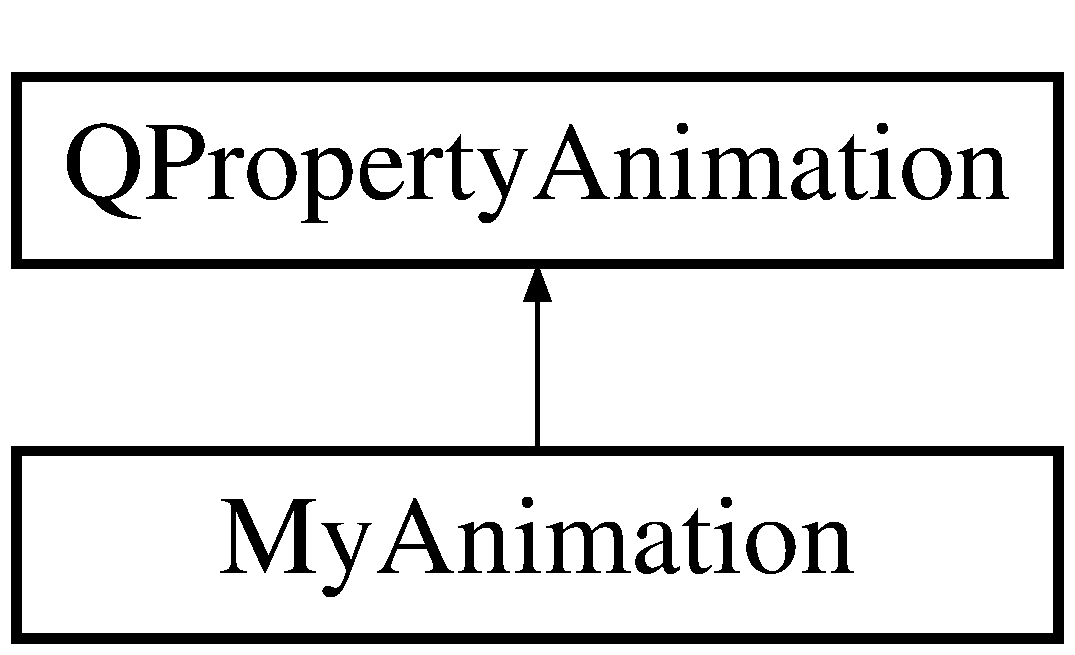
\includegraphics[height=2.000000cm]{class_my_animation}
\end{center}
\end{figure}
\subsection*{Public Member Functions}
\begin{DoxyCompactItemize}
\item 
\hyperlink{class_my_animation_afec096e94a98045d3cf87bf4dd247637}{My\-Animation} (Q\-Object $\ast$target, const Q\-Byte\-Array \&property\-Name)
\begin{DoxyCompactList}\small\item\em Konstruktor der Klasse \hyperlink{class_my_animation}{My\-Animation}. \end{DoxyCompactList}\item 
\hyperlink{class_my_animation_a68db19894ccd22277aff4c862a168cfe}{My\-Animation} (Q\-Object $\ast$parent)
\begin{DoxyCompactList}\small\item\em Konstruktor der Klasse \hyperlink{class_my_animation}{My\-Animation}. \end{DoxyCompactList}\item 
Q\-Point\-F \hyperlink{class_my_animation_a3e092d8b292b2317fc9136c0d78ab984}{get\-Old\-Vector} () const 
\begin{DoxyCompactList}\small\item\em Liefert den 2d-\/\-Richtungsvektor der Animation seit der letzten Änderung. \end{DoxyCompactList}\item 
void \hyperlink{class_my_animation_a3c83b6a68871f54a5a561c134db4cba2}{set\-Old\-Vector} (const Q\-Point\-F \&value)
\begin{DoxyCompactList}\small\item\em Speichert einen 2\-D-\/\-Vektor, der durch die letzte Änderung entstanden ist. \end{DoxyCompactList}\item 
Q\-Point\-F \hyperlink{class_my_animation_a6dddda03203449e45354405d14ffb436}{get\-Old\-Position} () const 
\begin{DoxyCompactList}\small\item\em Liefert die Position vor der letzten Änderung. \end{DoxyCompactList}\item 
void \hyperlink{class_my_animation_adb71d57fddec8dd3ef563f6f0b386710}{set\-Old\-Position} (const Q\-Point\-F \&value)
\begin{DoxyCompactList}\small\item\em Speichert die Position seit der letzten änderung. \end{DoxyCompactList}\end{DoxyCompactItemize}


\subsection{Constructor \& Destructor Documentation}
\hypertarget{class_my_animation_afec096e94a98045d3cf87bf4dd247637}{\index{My\-Animation@{My\-Animation}!My\-Animation@{My\-Animation}}
\index{My\-Animation@{My\-Animation}!MyAnimation@{My\-Animation}}
\subsubsection[{My\-Animation}]{\setlength{\rightskip}{0pt plus 5cm}My\-Animation\-::\-My\-Animation (
\begin{DoxyParamCaption}
\item[{Q\-Object $\ast$}]{target, }
\item[{const Q\-Byte\-Array \&}]{property\-Name}
\end{DoxyParamCaption}
)}}\label{class_my_animation_afec096e94a98045d3cf87bf4dd247637}


Konstruktor der Klasse \hyperlink{class_my_animation}{My\-Animation}. 


\begin{DoxyParams}{Parameters}
{\em target} & Q\-Object, das animiert werden soll\\
\hline
{\em property\-Name} & Property, die zur Animation benutzt werden soll\\
\hline
\end{DoxyParams}
\hypertarget{class_my_animation_a68db19894ccd22277aff4c862a168cfe}{\index{My\-Animation@{My\-Animation}!My\-Animation@{My\-Animation}}
\index{My\-Animation@{My\-Animation}!MyAnimation@{My\-Animation}}
\subsubsection[{My\-Animation}]{\setlength{\rightskip}{0pt plus 5cm}My\-Animation\-::\-My\-Animation (
\begin{DoxyParamCaption}
\item[{Q\-Object $\ast$}]{parent}
\end{DoxyParamCaption}
)}}\label{class_my_animation_a68db19894ccd22277aff4c862a168cfe}


Konstruktor der Klasse \hyperlink{class_my_animation}{My\-Animation}. 



\subsection{Member Function Documentation}
\hypertarget{class_my_animation_a6dddda03203449e45354405d14ffb436}{\index{My\-Animation@{My\-Animation}!get\-Old\-Position@{get\-Old\-Position}}
\index{get\-Old\-Position@{get\-Old\-Position}!MyAnimation@{My\-Animation}}
\subsubsection[{get\-Old\-Position}]{\setlength{\rightskip}{0pt plus 5cm}Q\-Point\-F My\-Animation\-::get\-Old\-Position (
\begin{DoxyParamCaption}
{}
\end{DoxyParamCaption}
) const}}\label{class_my_animation_a6dddda03203449e45354405d14ffb436}


Liefert die Position vor der letzten Änderung. 

\hypertarget{class_my_animation_a3e092d8b292b2317fc9136c0d78ab984}{\index{My\-Animation@{My\-Animation}!get\-Old\-Vector@{get\-Old\-Vector}}
\index{get\-Old\-Vector@{get\-Old\-Vector}!MyAnimation@{My\-Animation}}
\subsubsection[{get\-Old\-Vector}]{\setlength{\rightskip}{0pt plus 5cm}Q\-Point\-F My\-Animation\-::get\-Old\-Vector (
\begin{DoxyParamCaption}
{}
\end{DoxyParamCaption}
) const}}\label{class_my_animation_a3e092d8b292b2317fc9136c0d78ab984}


Liefert den 2d-\/\-Richtungsvektor der Animation seit der letzten Änderung. 

\hypertarget{class_my_animation_adb71d57fddec8dd3ef563f6f0b386710}{\index{My\-Animation@{My\-Animation}!set\-Old\-Position@{set\-Old\-Position}}
\index{set\-Old\-Position@{set\-Old\-Position}!MyAnimation@{My\-Animation}}
\subsubsection[{set\-Old\-Position}]{\setlength{\rightskip}{0pt plus 5cm}void My\-Animation\-::set\-Old\-Position (
\begin{DoxyParamCaption}
\item[{const Q\-Point\-F \&}]{value}
\end{DoxyParamCaption}
)}}\label{class_my_animation_adb71d57fddec8dd3ef563f6f0b386710}


Speichert die Position seit der letzten änderung. 

\hypertarget{class_my_animation_a3c83b6a68871f54a5a561c134db4cba2}{\index{My\-Animation@{My\-Animation}!set\-Old\-Vector@{set\-Old\-Vector}}
\index{set\-Old\-Vector@{set\-Old\-Vector}!MyAnimation@{My\-Animation}}
\subsubsection[{set\-Old\-Vector}]{\setlength{\rightskip}{0pt plus 5cm}void My\-Animation\-::set\-Old\-Vector (
\begin{DoxyParamCaption}
\item[{const Q\-Point\-F \&}]{value}
\end{DoxyParamCaption}
)}}\label{class_my_animation_a3c83b6a68871f54a5a561c134db4cba2}


Speichert einen 2\-D-\/\-Vektor, der durch die letzte Änderung entstanden ist. 



The documentation for this class was generated from the following files\-:\begin{DoxyCompactItemize}
\item 
myanimation.\-h\item 
merge.\-cpp\item 
myanimation.\-cpp\end{DoxyCompactItemize}

\hypertarget{class_my_field}{\section{My\-Field Class Reference}
\label{class_my_field}\index{My\-Field@{My\-Field}}
}


Klasse für das Spielbrett. Die Mehrfachvererbung ist für die Animation notwendig  




{\ttfamily \#include $<$myfield.\-h$>$}



Inheritance diagram for My\-Field\-:


Collaboration diagram for My\-Field\-:
\subsection*{Public Member Functions}
\begin{DoxyCompactItemize}
\item 
\hyperlink{class_my_field_a33ebf8426146babbc87906903a12aba0}{My\-Field} ()
\begin{DoxyCompactList}\small\item\em Konstruktor der Klasse \hyperlink{class_my_field}{My\-Field}. \end{DoxyCompactList}\end{DoxyCompactItemize}
\subsection*{Properties}
\begin{DoxyCompactItemize}
\item 
\hypertarget{class_my_field_aaed9208f84a77a212771fbaa848a31bd}{Q\-Point\-F {\bfseries pos}}\label{class_my_field_aaed9208f84a77a212771fbaa848a31bd}

\end{DoxyCompactItemize}


\subsection{Detailed Description}
Klasse für das Spielbrett. Die Mehrfachvererbung ist für die Animation notwendig 



\subsection{Constructor \& Destructor Documentation}
\hypertarget{class_my_field_a33ebf8426146babbc87906903a12aba0}{\index{My\-Field@{My\-Field}!My\-Field@{My\-Field}}
\index{My\-Field@{My\-Field}!MyField@{My\-Field}}
\subsubsection[{My\-Field}]{\setlength{\rightskip}{0pt plus 5cm}My\-Field\-::\-My\-Field (
\begin{DoxyParamCaption}
{}
\end{DoxyParamCaption}
)}}\label{class_my_field_a33ebf8426146babbc87906903a12aba0}


Konstruktor der Klasse \hyperlink{class_my_field}{My\-Field}. 



The documentation for this class was generated from the following files\-:\begin{DoxyCompactItemize}
\item 
myfield.\-h\item 
merge.\-cpp\item 
myfield.\-cpp\end{DoxyCompactItemize}

\hypertarget{class_my_gradient}{\section{My\-Gradient Class Reference}
\label{class_my_gradient}\index{My\-Gradient@{My\-Gradient}}
}
Inheritance diagram for My\-Gradient\-:\begin{figure}[H]
\begin{center}
\leavevmode
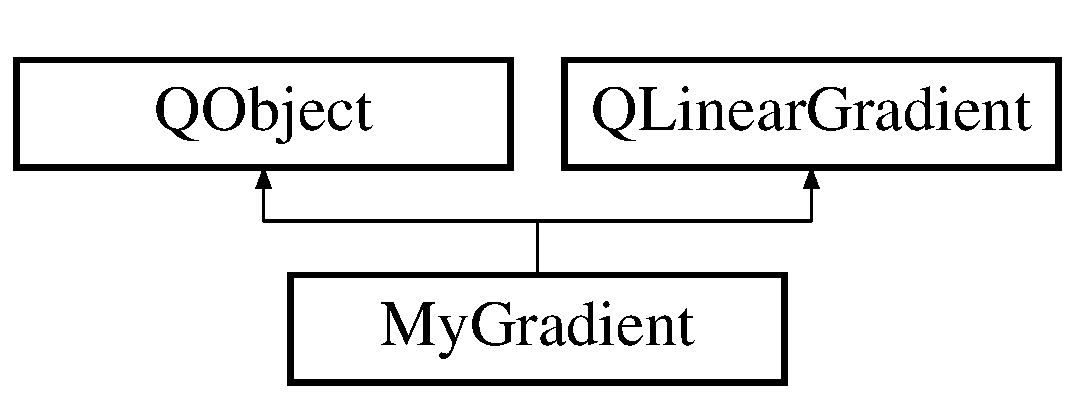
\includegraphics[height=2.000000cm]{class_my_gradient}
\end{center}
\end{figure}
\subsection*{Public Member Functions}
\begin{DoxyCompactItemize}
\item 
\hypertarget{class_my_gradient_a27908adf6a6414a655fcdeace0953302}{W\-R\-I\-T\-E set\-Middle()) public {\bfseries My\-Gradient} (Q\-Point p, Q\-Point q)}\label{class_my_gradient_a27908adf6a6414a655fcdeace0953302}

\item 
\hypertarget{class_my_gradient_ae4ff6baad026510ca45d7a9f8ffda66a}{float {\bfseries get\-Middle} ()}\label{class_my_gradient_ae4ff6baad026510ca45d7a9f8ffda66a}

\item 
\hypertarget{class_my_gradient_a1656afe4362af1975765577cfae0cca4}{void {\bfseries set\-Middle} (float value)}\label{class_my_gradient_a1656afe4362af1975765577cfae0cca4}

\item 
\hypertarget{class_my_gradient_a2623282273f1ea70ad7fa7ce2a413f66}{void {\bfseries set\-C\-Start} (const Q\-Color \&value, float s)}\label{class_my_gradient_a2623282273f1ea70ad7fa7ce2a413f66}

\item 
\hypertarget{class_my_gradient_a361ab9506f1206105e256f7c0003beff}{void {\bfseries set\-C\-Middle} (const Q\-Color \&value, float m)}\label{class_my_gradient_a361ab9506f1206105e256f7c0003beff}

\item 
\hypertarget{class_my_gradient_aebcbe44cd5b4bcab9c02d02ddf3557c1}{void {\bfseries set\-C\-End} (const Q\-Color \&value, float e)}\label{class_my_gradient_aebcbe44cd5b4bcab9c02d02ddf3557c1}

\end{DoxyCompactItemize}
\subsection*{Properties}
\begin{DoxyCompactItemize}
\item 
\hypertarget{class_my_gradient_ac84c06b398f8b56bfbb7df2d92823ba9}{float {\bfseries Middle}}\label{class_my_gradient_ac84c06b398f8b56bfbb7df2d92823ba9}

\item 
\hypertarget{class_my_gradient_a7cf03f924418dcc57e2e03ed2f27fc88}{Q\-Color {\bfseries c\-Start}}\label{class_my_gradient_a7cf03f924418dcc57e2e03ed2f27fc88}

\item 
\hypertarget{class_my_gradient_a1680b943f4644e745fe1543461343234}{Q\-Color {\bfseries c\-Middle}}\label{class_my_gradient_a1680b943f4644e745fe1543461343234}

\item 
\hypertarget{class_my_gradient_a5970c7e15913cb02a35433891d969a94}{Q\-Color {\bfseries c\-End}}\label{class_my_gradient_a5970c7e15913cb02a35433891d969a94}

\item 
\hypertarget{class_my_gradient_a2afe04c6cbf3e2abbbfb2987707cc7fb}{float {\bfseries start}}\label{class_my_gradient_a2afe04c6cbf3e2abbbfb2987707cc7fb}

\item 
\hypertarget{class_my_gradient_a96e799bbd6ca5334eaa89d3c952272bd}{float {\bfseries middle}}\label{class_my_gradient_a96e799bbd6ca5334eaa89d3c952272bd}

\item 
\hypertarget{class_my_gradient_ab6ce1fa1f132699b9d2302c327afdc16}{float {\bfseries end}}\label{class_my_gradient_ab6ce1fa1f132699b9d2302c327afdc16}

\end{DoxyCompactItemize}


The documentation for this class was generated from the following files\-:\begin{DoxyCompactItemize}
\item 
mygradient.\-h\item 
merge.\-cpp\item 
mygradient.\-cpp\end{DoxyCompactItemize}

\hypertarget{class_my_graphics_scene}{\section{My\-Graphics\-Scene Class Reference}
\label{class_my_graphics_scene}\index{My\-Graphics\-Scene@{My\-Graphics\-Scene}}
}
Inheritance diagram for My\-Graphics\-Scene\-:\begin{figure}[H]
\begin{center}
\leavevmode
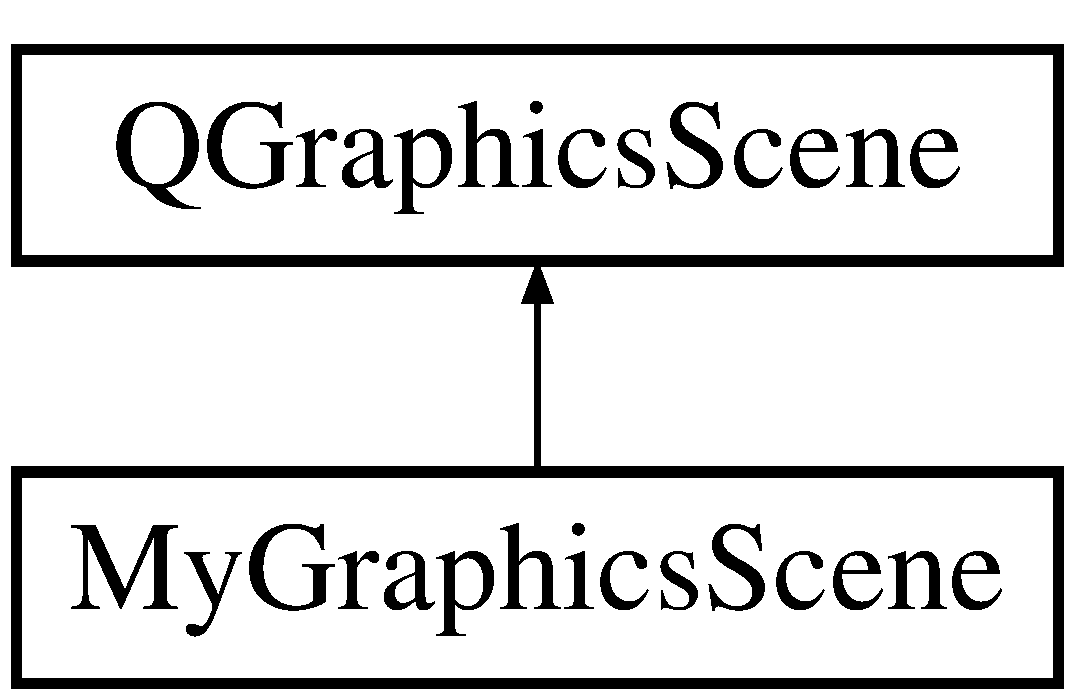
\includegraphics[height=2.000000cm]{class_my_graphics_scene}
\end{center}
\end{figure}
\subsection*{Public Slots}
\begin{DoxyCompactItemize}
\item 
void \hyperlink{class_my_graphics_scene_ae13be07253c9d3ff11c336c09cd89daf}{bounce\-Sound} (Q\-Variant v)
\begin{DoxyCompactList}\small\item\em Slot für das Abspielen von Bounce geräuschen. Bei jeder Richtungsänderung des Objekts kann zur entsprechenden Easingkurve das geräusch abgespielt werden. Die Soundwiedergabe ist nicht implementiert. \end{DoxyCompactList}\item 
void \hyperlink{class_my_graphics_scene_a47693d863886396ee37b3bec05ac341f}{animate\-Victory} ()
\begin{DoxyCompactList}\small\item\em Signalisiert dem Spieler den Endzustand des Spiels durch eine Animation \end{DoxyCompactList}\end{DoxyCompactItemize}
\subsection*{Public Member Functions}
\begin{DoxyCompactItemize}
\item 
\hyperlink{class_my_graphics_scene_a0a9622d196f6ea758f119faddf37caac}{My\-Graphics\-Scene} (Q\-Object $\ast$parent, \hyperlink{class_connect_four}{Connect\-Four} $\ast$game, int selected\-Design)
\begin{DoxyCompactList}\small\item\em Konstruktor der Klasse My\-Graphic\-Scene. Liefert eine Instanz zur Darstellung des Connect Four-\/\-Spiels \end{DoxyCompactList}\item 
\hyperlink{class_connect_four}{Connect\-Four} $\ast$ \hyperlink{class_my_graphics_scene_a7883bc1ffdb2cf3834179de0d3f14843}{get\-Cfgame} () const 
\begin{DoxyCompactList}\small\item\em Liefert einen Zeiger auf die Instanz der Spielklasse \end{DoxyCompactList}\item 
void \hyperlink{class_my_graphics_scene_a89bb2786bb7a9a4c13a37ad1296ffaf0}{set\-Cfgame} (\hyperlink{class_connect_four}{Connect\-Four} $\ast$value)
\begin{DoxyCompactList}\small\item\em Setzt die Instanz der Spielklasse fest \end{DoxyCompactList}\item 
float \hyperlink{class_my_graphics_scene_ab2dc3b23ea848b5f081939d569b16774}{scalar\-Product} (Q\-Point\-F u, Q\-Point\-F v)
\begin{DoxyCompactList}\small\item\em Liefert das Skalarprodukt zweier 2d-\/\-Vektoren \end{DoxyCompactList}\end{DoxyCompactItemize}
\subsection*{Protected Member Functions}
\begin{DoxyCompactItemize}
\item 
virtual void \hyperlink{class_my_graphics_scene_a65a5dabb614e22ae4a4b48d9f2faffdc}{mouse\-Release\-Event} (Q\-Graphics\-Scene\-Mouse\-Event $\ast$event)
\begin{DoxyCompactList}\small\item\em Fängt den Spieler click ab, der seine Spalte durch anclicken wählen soll. \end{DoxyCompactList}\item 
virtual void \hyperlink{class_my_graphics_scene_a174dd0911afadc8f637a5ebf6f5b9b0c}{resize\-Event} (Q\-Resize\-Event $\ast$event)
\begin{DoxyCompactList}\small\item\em Fängt das Resize Event ab und berechnet die Spaltenbreite \end{DoxyCompactList}\end{DoxyCompactItemize}


\subsection{Constructor \& Destructor Documentation}
\hypertarget{class_my_graphics_scene_a0a9622d196f6ea758f119faddf37caac}{\index{My\-Graphics\-Scene@{My\-Graphics\-Scene}!My\-Graphics\-Scene@{My\-Graphics\-Scene}}
\index{My\-Graphics\-Scene@{My\-Graphics\-Scene}!MyGraphicsScene@{My\-Graphics\-Scene}}
\subsubsection[{My\-Graphics\-Scene}]{\setlength{\rightskip}{0pt plus 5cm}My\-Graphics\-Scene\-::\-My\-Graphics\-Scene (
\begin{DoxyParamCaption}
\item[{Q\-Object $\ast$}]{parent, }
\item[{{\bf Connect\-Four} $\ast$}]{game, }
\item[{int}]{selected\-Design}
\end{DoxyParamCaption}
)\hspace{0.3cm}{\ttfamily [explicit]}}}\label{class_my_graphics_scene_a0a9622d196f6ea758f119faddf37caac}


Konstruktor der Klasse My\-Graphic\-Scene. Liefert eine Instanz zur Darstellung des Connect Four-\/\-Spiels 


\begin{DoxyParams}{Parameters}
{\em parent} & Parentobjekt\\
\hline
{\em game} & Instanz des Spiels\\
\hline
{\em game} & gewähltes Design\\
\hline
\end{DoxyParams}


\subsection{Member Function Documentation}
\hypertarget{class_my_graphics_scene_a47693d863886396ee37b3bec05ac341f}{\index{My\-Graphics\-Scene@{My\-Graphics\-Scene}!animate\-Victory@{animate\-Victory}}
\index{animate\-Victory@{animate\-Victory}!MyGraphicsScene@{My\-Graphics\-Scene}}
\subsubsection[{animate\-Victory}]{\setlength{\rightskip}{0pt plus 5cm}void My\-Graphics\-Scene\-::animate\-Victory (
\begin{DoxyParamCaption}
{}
\end{DoxyParamCaption}
)\hspace{0.3cm}{\ttfamily [slot]}}}\label{class_my_graphics_scene_a47693d863886396ee37b3bec05ac341f}


Signalisiert dem Spieler den Endzustand des Spiels durch eine Animation 

\hypertarget{class_my_graphics_scene_ae13be07253c9d3ff11c336c09cd89daf}{\index{My\-Graphics\-Scene@{My\-Graphics\-Scene}!bounce\-Sound@{bounce\-Sound}}
\index{bounce\-Sound@{bounce\-Sound}!MyGraphicsScene@{My\-Graphics\-Scene}}
\subsubsection[{bounce\-Sound}]{\setlength{\rightskip}{0pt plus 5cm}void My\-Graphics\-Scene\-::bounce\-Sound (
\begin{DoxyParamCaption}
\item[{Q\-Variant}]{v}
\end{DoxyParamCaption}
)\hspace{0.3cm}{\ttfamily [slot]}}}\label{class_my_graphics_scene_ae13be07253c9d3ff11c336c09cd89daf}


Slot für das Abspielen von Bounce geräuschen. Bei jeder Richtungsänderung des Objekts kann zur entsprechenden Easingkurve das geräusch abgespielt werden. Die Soundwiedergabe ist nicht implementiert. 


\begin{DoxyParams}{Parameters}
{\em v} & Sender des Signals\\
\hline
\end{DoxyParams}
\hypertarget{class_my_graphics_scene_a7883bc1ffdb2cf3834179de0d3f14843}{\index{My\-Graphics\-Scene@{My\-Graphics\-Scene}!get\-Cfgame@{get\-Cfgame}}
\index{get\-Cfgame@{get\-Cfgame}!MyGraphicsScene@{My\-Graphics\-Scene}}
\subsubsection[{get\-Cfgame}]{\setlength{\rightskip}{0pt plus 5cm}{\bf Connect\-Four} $\ast$ My\-Graphics\-Scene\-::get\-Cfgame (
\begin{DoxyParamCaption}
{}
\end{DoxyParamCaption}
) const}}\label{class_my_graphics_scene_a7883bc1ffdb2cf3834179de0d3f14843}


Liefert einen Zeiger auf die Instanz der Spielklasse 

\hypertarget{class_my_graphics_scene_a65a5dabb614e22ae4a4b48d9f2faffdc}{\index{My\-Graphics\-Scene@{My\-Graphics\-Scene}!mouse\-Release\-Event@{mouse\-Release\-Event}}
\index{mouse\-Release\-Event@{mouse\-Release\-Event}!MyGraphicsScene@{My\-Graphics\-Scene}}
\subsubsection[{mouse\-Release\-Event}]{\setlength{\rightskip}{0pt plus 5cm}void My\-Graphics\-Scene\-::mouse\-Release\-Event (
\begin{DoxyParamCaption}
\item[{Q\-Graphics\-Scene\-Mouse\-Event $\ast$}]{event}
\end{DoxyParamCaption}
)\hspace{0.3cm}{\ttfamily [protected]}, {\ttfamily [virtual]}}}\label{class_my_graphics_scene_a65a5dabb614e22ae4a4b48d9f2faffdc}


Fängt den Spieler click ab, der seine Spalte durch anclicken wählen soll. 


\begin{DoxyParams}{Parameters}
{\em event} & enthält die clickinformationen\\
\hline
\end{DoxyParams}
\hypertarget{class_my_graphics_scene_a174dd0911afadc8f637a5ebf6f5b9b0c}{\index{My\-Graphics\-Scene@{My\-Graphics\-Scene}!resize\-Event@{resize\-Event}}
\index{resize\-Event@{resize\-Event}!MyGraphicsScene@{My\-Graphics\-Scene}}
\subsubsection[{resize\-Event}]{\setlength{\rightskip}{0pt plus 5cm}void My\-Graphics\-Scene\-::resize\-Event (
\begin{DoxyParamCaption}
\item[{Q\-Resize\-Event $\ast$}]{event}
\end{DoxyParamCaption}
)\hspace{0.3cm}{\ttfamily [protected]}, {\ttfamily [virtual]}}}\label{class_my_graphics_scene_a174dd0911afadc8f637a5ebf6f5b9b0c}


Fängt das Resize Event ab und berechnet die Spaltenbreite 

\hypertarget{class_my_graphics_scene_ab2dc3b23ea848b5f081939d569b16774}{\index{My\-Graphics\-Scene@{My\-Graphics\-Scene}!scalar\-Product@{scalar\-Product}}
\index{scalar\-Product@{scalar\-Product}!MyGraphicsScene@{My\-Graphics\-Scene}}
\subsubsection[{scalar\-Product}]{\setlength{\rightskip}{0pt plus 5cm}float My\-Graphics\-Scene\-::scalar\-Product (
\begin{DoxyParamCaption}
\item[{Q\-Point\-F}]{u, }
\item[{Q\-Point\-F}]{v}
\end{DoxyParamCaption}
)}}\label{class_my_graphics_scene_ab2dc3b23ea848b5f081939d569b16774}


Liefert das Skalarprodukt zweier 2d-\/\-Vektoren 

\hypertarget{class_my_graphics_scene_a89bb2786bb7a9a4c13a37ad1296ffaf0}{\index{My\-Graphics\-Scene@{My\-Graphics\-Scene}!set\-Cfgame@{set\-Cfgame}}
\index{set\-Cfgame@{set\-Cfgame}!MyGraphicsScene@{My\-Graphics\-Scene}}
\subsubsection[{set\-Cfgame}]{\setlength{\rightskip}{0pt plus 5cm}void My\-Graphics\-Scene\-::set\-Cfgame (
\begin{DoxyParamCaption}
\item[{{\bf Connect\-Four} $\ast$}]{value}
\end{DoxyParamCaption}
)}}\label{class_my_graphics_scene_a89bb2786bb7a9a4c13a37ad1296ffaf0}


Setzt die Instanz der Spielklasse fest 



The documentation for this class was generated from the following files\-:\begin{DoxyCompactItemize}
\item 
mygraphicsscene.\-h\item 
merge.\-cpp\item 
mygraphicsscene.\-cpp\end{DoxyCompactItemize}

\hypertarget{class_my_graphics_view}{\section{My\-Graphics\-View Class Reference}
\label{class_my_graphics_view}\index{My\-Graphics\-View@{My\-Graphics\-View}}
}


Parentobjekt für die Spielszene. Fängt Tastendrücke ab und achtet auf die Seitenverhältnisse.  




{\ttfamily \#include $<$mygraphicsview.\-h$>$}



Inheritance diagram for My\-Graphics\-View\-:


Collaboration diagram for My\-Graphics\-View\-:
\subsection*{Public Member Functions}
\begin{DoxyCompactItemize}
\item 
\hyperlink{class_my_graphics_view_ae55142e35dbafe5f76fa9fb5b7563ec8}{My\-Graphics\-View} (Q\-Widget $\ast$parent=0, \hyperlink{class_data_base_access_class}{Data\-Base\-Access\-Class} $\ast$dao=0)
\begin{DoxyCompactList}\small\item\em Konstruktor der Klasse \hyperlink{class_my_graphics_view}{My\-Graphics\-View}. \end{DoxyCompactList}\end{DoxyCompactItemize}
\subsection*{Protected Member Functions}
\begin{DoxyCompactItemize}
\item 
virtual void \hyperlink{class_my_graphics_view_a93b12d4302622836f0150a8b56ff3c9f}{resize\-Event} (Q\-Resize\-Event $\ast$event)
\begin{DoxyCompactList}\small\item\em Zum erhalt der Seitenverhältnisse \end{DoxyCompactList}\item 
virtual void \hyperlink{class_my_graphics_view_a9816bdd436d67c34f1b0d8feed15d47d}{key\-Press\-Event} (Q\-Key\-Event $\ast$event)
\begin{DoxyCompactList}\small\item\em Fängt benutzereingaben ab. \mbox{[}Ss\mbox{]} speichert das Spiel \mbox{[}Ff\mbox{]} aktiviert und deaktiviert den Fullscreen modus \end{DoxyCompactList}\end{DoxyCompactItemize}


\subsection{Detailed Description}
Parentobjekt für die Spielszene. Fängt Tastendrücke ab und achtet auf die Seitenverhältnisse. 



\subsection{Constructor \& Destructor Documentation}
\hypertarget{class_my_graphics_view_ae55142e35dbafe5f76fa9fb5b7563ec8}{\index{My\-Graphics\-View@{My\-Graphics\-View}!My\-Graphics\-View@{My\-Graphics\-View}}
\index{My\-Graphics\-View@{My\-Graphics\-View}!MyGraphicsView@{My\-Graphics\-View}}
\subsubsection[{My\-Graphics\-View}]{\setlength{\rightskip}{0pt plus 5cm}My\-Graphics\-View\-::\-My\-Graphics\-View (
\begin{DoxyParamCaption}
\item[{Q\-Widget $\ast$}]{parent = {\ttfamily 0}, }
\item[{{\bf Data\-Base\-Access\-Class} $\ast$}]{dao = {\ttfamily 0}}
\end{DoxyParamCaption}
)\hspace{0.3cm}{\ttfamily [explicit]}}}\label{class_my_graphics_view_ae55142e35dbafe5f76fa9fb5b7563ec8}


Konstruktor der Klasse \hyperlink{class_my_graphics_view}{My\-Graphics\-View}. 


\begin{DoxyParams}{Parameters}
{\em parent} & Parentobjekt\\
\hline
{\em dao} & Objekt zum Zugriff auf die Spieledatenbank\\
\hline
\end{DoxyParams}


\subsection{Member Function Documentation}
\hypertarget{class_my_graphics_view_a9816bdd436d67c34f1b0d8feed15d47d}{\index{My\-Graphics\-View@{My\-Graphics\-View}!key\-Press\-Event@{key\-Press\-Event}}
\index{key\-Press\-Event@{key\-Press\-Event}!MyGraphicsView@{My\-Graphics\-View}}
\subsubsection[{key\-Press\-Event}]{\setlength{\rightskip}{0pt plus 5cm}void My\-Graphics\-View\-::key\-Press\-Event (
\begin{DoxyParamCaption}
\item[{Q\-Key\-Event $\ast$}]{event}
\end{DoxyParamCaption}
)\hspace{0.3cm}{\ttfamily [protected]}, {\ttfamily [virtual]}}}\label{class_my_graphics_view_a9816bdd436d67c34f1b0d8feed15d47d}


Fängt benutzereingaben ab. \mbox{[}Ss\mbox{]} speichert das Spiel \mbox{[}Ff\mbox{]} aktiviert und deaktiviert den Fullscreen modus 



Here is the call graph for this function\-:


\hypertarget{class_my_graphics_view_a93b12d4302622836f0150a8b56ff3c9f}{\index{My\-Graphics\-View@{My\-Graphics\-View}!resize\-Event@{resize\-Event}}
\index{resize\-Event@{resize\-Event}!MyGraphicsView@{My\-Graphics\-View}}
\subsubsection[{resize\-Event}]{\setlength{\rightskip}{0pt plus 5cm}void My\-Graphics\-View\-::resize\-Event (
\begin{DoxyParamCaption}
\item[{Q\-Resize\-Event $\ast$}]{event}
\end{DoxyParamCaption}
)\hspace{0.3cm}{\ttfamily [protected]}, {\ttfamily [virtual]}}}\label{class_my_graphics_view_a93b12d4302622836f0150a8b56ff3c9f}


Zum erhalt der Seitenverhältnisse 



The documentation for this class was generated from the following files\-:\begin{DoxyCompactItemize}
\item 
mygraphicsview.\-h\item 
merge.\-cpp\item 
mygraphicsview.\-cpp\end{DoxyCompactItemize}

%--- End generated contents ---

% Index
\newpage
\phantomsection
\addcontentsline{toc}{chapter}{Index}
\printindex

\end{document}
